\documentclass{article}
\usepackage[utf8]{inputenc}
\usepackage[spanish]{babel} 
\renewcommand{\spanishtablename}{Tabla} 
\spanishdecimal{.}
\usepackage{verbatim}
\usepackage{amssymb}
\usepackage{wrapfig}
\usepackage{graphicx}
\usepackage{mathtools}
\usepackage{float}
\usepackage{siunitx}
\renewcommand{\thefootnote}{\arabic{fotnote}}
\setlength{\parskip}{\baselineskip} 
\usepackage{pdfpages}

\begin{document}

\begin{titlepage}

\begin{center}
\vspace*{0.10in}
\begin{figure}
\raggedleft

\includegraphics[scale=0.12]{unam.png}
\hspace{7.2cm}
\raggedright
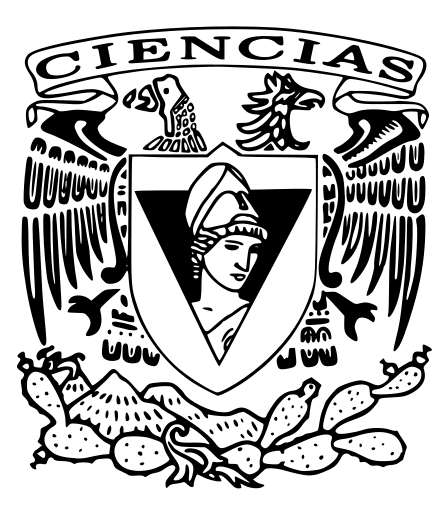
\includegraphics[scale=0.15]{fac.png}    
\end{figure}
\vspace*{0.5in}
UNIVERSIDAD NACIONAL AUTÓNOMA DE MÉXICO\\
\vspace*{0.2in}
FACULTAD DE CIENCIAS \\
\vspace*{0.5in}
\begin{large}
Laboratorio de Calor, Ondas y Fluidos\\
\end{large}
\vspace*{0.2in}
\begin{Large}
\textbf{Práctica 0} \\
\textbf{Mediciones} \\
\end{Large}
\vspace*{0.3in}
\vspace*{0.3in}
\rule{80mm}{0.1mm}\\
\vspace*{0.1in}
\begin{large}
Profesor:  Quintanar Robles, Luis  \\
Ayudante: Quintanar Cortés, Luis Enrique \\
Mesa 1\\
Alumnos: León Arenal Sebastian.\\
Robledo Ibarra Emiliano. \\
Toledo Castañeda, Akim Tarik.\\

\end{large}
\end{center}
\end{titlepage}


\section*{\centering{Resumen}}
    Se midió la  longitud de la mesa del laboratorio con cuatro instrumentos de resolución distinta, se calculó el volumen de dos cuerpos (uno regular y uno irregular) con una probeta y agua, se obtuvo la aceleración debida a la gravedad por medio de un péndulo. Resalta el hecho de contar con longitudes similares pero no idénticas en la longitud de la mesa. Además, se calculó una aceleración debida a la gravedad ciertamente por debajo del valor esperado $(9.3\pm0.8)m/s^2$. Sin embargo, el análisis de incertidumbres y los instrumentos de medición permiten darle certeza a los datos encontrados y justificar (como en el caso de $g$) las diferencias entre los datos obtenidos y los esperados teóricamente.


%%%%%%%%%%%%%%%%%%%%%%%%%%%%%%%%%%%%%%%%%%%%%%%%%%%%%%%%%%%%%%%%%%%%%%%%%%%%
\section{Introducción}

Las mediciones son una forma de conocer nuestro alrededor, gracias a ellas podemos describir y cuantificar aquellos aspectos que, como experimentales, nos interesan; no es posible estudiar un fenómeno físico sin hacer dichas mediciones, de manera que aprender a realizarlas correctamente es un punto clave que todo físico debe conocer.Es necesario aprender que toda medición tiene una incertidumbre asociada que indica la fiabilidad de la misma. También indica que tan buenas son las técnicas y los instrumentos utilizados para la medición.

La práctica consistió en medir volumen, longitud, altura y la constante de gravedad $g$ con distintos instrumentos y técnicas con el fin de conocer las incertidumbres asociadas y su propagación. Se midió el largo de una mesa, la altura de un rebote, el volumen de un objeto regular y el de uno irregular y el periodo de un péndulo. Para el caso de las longitudes variaron entre tipos de mediciones (directa e indirecta) debido al tamaño del instrumento; en cuanto al volumen, se partió de dos formas indirectas; la primera fue que al elegir un cubo su volumen está determinado por la ecuación: $l^3$. La segunda de el hecho de que cualquier objeto sumergido en agua aumenta el nivel de la misma y midiendo el volumen desplazado es como podemos averiguar el volumen del objeto sumergido.

Durante las mediciones se formularon hipótesis que sirvieron para simplificar los resultados. En primer lugar, se despreció la contracción/dilatación causada por la temperatura tanto en los objetos a medir como en los instrumentos de medición. La segunda hipótesis que se utilizó fue referente al periodo del péndulo . Un péndulo pierde energía conforme el tiempo debido a la fricción con el aire; sin embargo, se puede observar un periodo constante en un intervalo de tiempo corto.Para ángulos pequeños y considerando un péndulo simple, podemos aproximar el periodo con la ecuación $T = 2\pi \sqrt{l/g}$. 

%%%%%%%%%%%%%%%%%%%%%%%%%%%%%%%%%%%%%%%%%%%%%%%%%%%%%%%%%%%%%%%%%%%%%%%%%%%%

\section{Procedimiento.}
Se consideran cuatro sub-procedimientos:  medir la longitud de una mesa, encontrar una altura máxima $h$ después del segundo rebote  de una pelota en caída libre, calcular el valor de la aceleración de la gravedad por medio del periodo de un péndulo  y encontrar un volumen determinado. 
%%%%%%%%%%%%%%%%%%%%%%%%%%%%%%%%%%%%%%%%%%%%%%%%%%%%%%%%%%%%%%%%%%%%%%%%%%%%
\subsection{Longitud de la mesa.}
En esta sección se hablará las mediciones de la longitud de la mesa por cuatro objetos distintos. Algunos de los instrumentos de medición no tenían la dimensión necesaria para calcular por sí solos el largo total. Cuando este fue el caso, se hizo la máxima medición del instrumento, se marcó la mesa en ese punto y se colocó el mismo instrumento a partir de dicha marca. Esto se repitió hasta tener la medida completa. Se midió el largo con:
\begin{itemize}
  \item Flexómetro.
  \item Vernier.
  \item Regla de aluminio.
  \item Regla de madera.
\end{itemize}

\subsubsection{Flexómetro}
En este caso debido a que el instrumento consta de una longitud lo suficientemente grande como para realizar la medida, sólo se tuvo que colocar el extremo del flexómetro fijo en el borde de la mesa y mantener recta la banda metálica para obtener la medida directa.Se le asocia una incertidumbre igual a la mitad de la minima medida registrada en el instrumento, es decir $\pm0.05cm.$

\begin{figure}[H]
    \centering
    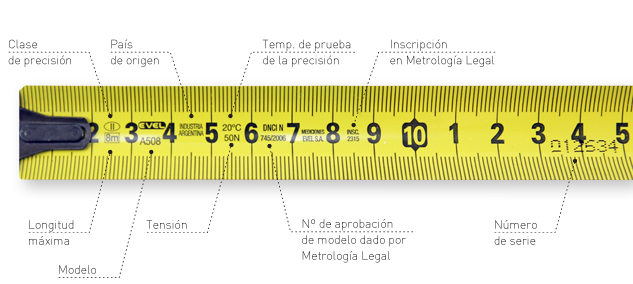
\includegraphics[width=7cm]{cert.png}%
    \caption{Diagrama de un flexómetro.}%
\end{figure}
cent
\subsubsection{Regla de madera}
La regla utilizada fue un metro de madera con divisiones cada centímetro. La mesa es más larga que la regla, entonces se tuvo que utilizar el instrumento dos veces, por lo que la incertidumbre se propaga. Las incertidumbres de una medida directa se suman, por lo tanto se le asocio a esta medida una incertidumbre de $(\pm0.05cm) + (\pm 0.05cm) = \pm 0.1 cm.$

\begin{figure}[H]
    \centering
    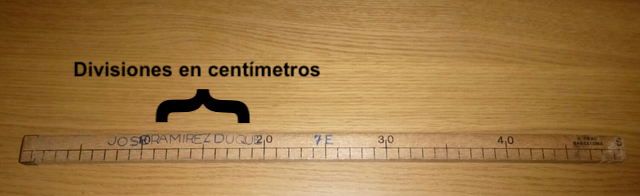
\includegraphics[width=7cm]{Untitled.png}%
    \caption{Diagrama de una regla de madera (representación).}%
\end{figure}

\subsubsection{Regla de aluminio}
Para este objeto se tuvo que calcular la longitud utilizando varias veces el instrumento de manera que para obtener la medida se sumaron las mediciones hasta obtener la final; como la regla mide $( 30.00 \pm 0.05 )$ cm, se sumó siete veces por lo cual la incertidumbre de la medida será de  $7*(0.05cm) = 0.35cm$.

\begin{figure}[H]
    \centering
    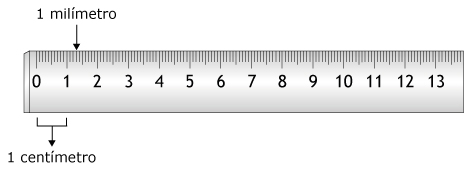
\includegraphics[width=7cm]{act31_2.jpg}%
    \caption{Diagrama de una regla de aluminio.}%
\end{figure}

\subsubsection{Vernier}
Para esta medición se tuvo que calcular la longitud utilizando varias veces el instrumento de manera que para obtener la medida se sumaron las mediciones hasta obtener la final; el vernier constaba de una resolución de $\frac{1}{20} mm$. Se decidió utilizar las mordazas para medidas externas en toda la medición y se utilizó fijando una apertura inicial de $( 10.000 \pm 0.002 )$ cm y se mantuvo así para facilitar la repetición de dicho patrón, de forma que al finalizar la medición se realizaron 19 repeticiones del patrón mencionado y una última para ajustarlo a la parte final. Así pues, la incertidumbre asociada a esta medida es de $\pm 0.038 cm$

\begin{figure}[H]
    \centering
    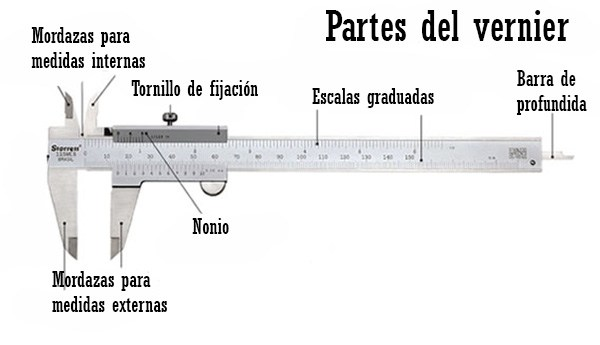
\includegraphics[width=7cm]{partes-vernier.jpg}%
    \caption{Diagrama de un vernier}%
\end{figure}



\subsection{Altura del rebote de una pelota}
Para cuantificar la altura que alcanza con el segundo rebote se optó por grabar el objeto mientras caía en cámara lenta. La [Figura 5] describe el montaje para medir la altura. Se soltó siempre desde una altura inicial $h_i = (80 \pm 0.5)$ cm. El experimento se repitió 6 veces; una vez medidas las alturas, se promediaron para obtener $\bar{h}$ y por medio de la desviación estándar se le otorgó una incertidumbre adecuada.

\begin{figure}[H]
    \centering
    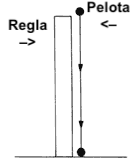
\includegraphics[width=3cm]{tiro.png}%
    \caption{Diagrama del sistema para medir el segundo rebote.}%
\end{figure}

\subsection{Valor de $g$}
Para medir la aceleración debida a la gravedad de la Tierra se utilizó un péndulo simple [Figura 6] que por longitud tuvo $(66.00 \pm 0.05) cm$; una plomada esférica hizo el papel de masa puntual y se montó con un soporte universal que sujetaba las varillas que eran perpendiculares entre sí.

Se fijaron ambas varillas para evitar movimientos que alteraran la medición. Además se optó por utilizar un mismo movimiento del péndulo es decir se usó un único movimiento del péndulo de manera que toda medida extraída del mismo proviene del mismo sistema en sus condiciones intactas; es necesario mencionar que con la ayuda de un transportador se verificó un ángulo de amplitud inicial menor a 15º que es un requisito de hipótesis para la relación utilizada. En lo referente al cálculo de la constante deseada, se midieron doce oscilaciones (periodos) y un promedio con con sus respectivas incertidumbre  para después aplicar la fórmula: $g = \frac{4\pi^2l}{T}$.

Después de la obtención del periodo se ocupó el método de propagación de incertidumbres de la fórmula antes mencionada y se encontró que la incertidumbre está dada por:

$$ dg = \left| \frac{4\pi^2}{T}\right| dl + \left| \frac{-4\pi^2}{T^2}\right| dT $$

\begin{figure}[H]
    \centering
    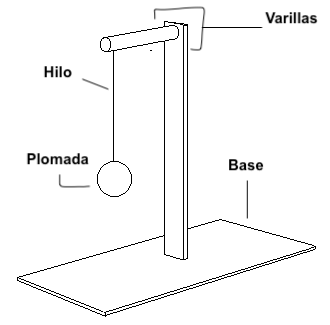
\includegraphics[width=5cm]{pendulo.png}%
    \caption{Diagrama del sistema para medir el periodo de un péndulo.}%
\end{figure}


\subsection{Volumen de dos objetos.}
 Para el objeto regular se ocupó un cubo, se midió uno de sus lados y luego se ocupó la relación $V = l^3$ y finalmente a este dato obtenido se le agregó la incertidumbre de la propagación diferenciando $V$: $\frac{\partial V}{\partial l} = 3l^2$ con $dl = 0.002$cm. La otra forma de medición consistió en llenar una probeta de agua hasta la marca base de 200 ml y posteriormente sumergir el objeto para poder obtener la diferencia entre volúmenes; la incertidumbre asignada será la suma de la incertidumbre inherente a la probeta.

En cuanto al objeto irregular se ocupó el mismo método de medición con la probeta.

% % % % % % % % % Completar lo del volumen










\section{Resultados.}
A continuación se muestran los resultados finales de todas las mediciones.

\subsection{Longitud del largo de la mesa.}
\begin{itemize}
  \item Flexómetro: $ L_{flexometro} =  ( 196.90 \pm 0.05 )$ cm.
  \item Regla de madera: $ L_{madera} = ( 197 \pm 1 )$ cm.
  \item Regla de aluminio: $ L_{aluminio} = ( 197.2 \pm 0.4 )$ cm.
  \item Vernier: $ L_{vernier} = ( 197.7 \pm 0.4 ) $ cm.
\end{itemize}

\subsection{Altura del segundo rebote.}
Ya que se repitió seis veces el experimento, se muestra la tabla siguiente:
\begin{table}[H]
  \centering
    \begin{tabular}{|c|c|c|} \hline
    Intento & Altura [cm] & Incertidumbre [cm] \\ \hline
    1º    & 46.0    & 0.5 \\ \hline
    2º    & 35.0    & 0.5 \\ \hline
    3º    & 37.0    & 0.5 \\ \hline
    4º    & 45.0    & 0.5 \\ \hline
    5º    & 47.0    & 0.5 \\ \hline
    6º    & 42.0    & 0.5 \\ \hline
    \end{tabular}%
\caption{Alturas del segundo rebote de una pelota.}
\end{table}%

Y se obtuvo: $h_{prom} = (42 \pm 5)$ cm.

\subsection{Valor de $g$.}
Gracias a la función: $T = 2\pi \sqrt{l/g}$. Podemos obtener $g = \frac{4\pi^2l}{T}$

% Table generated by Excel2LaTeX from sheet 'Hoja 1'
\begin{table}[H]
  \centering
    \begin{tabular}{|c|c|} \hline
    Medición & Periodo [s] \\ \hline
    1     & 1.63 \\ \hline
    2     & 1.65 \\ \hline
    3     & 1.79 \\ \hline
    4     & 1.66 \\ \hline
    5     & 1.51 \\ \hline
    6     & 1.68 \\ \hline
    7     & 1.71 \\ \hline
    8     & 1.59 \\ \hline
    9     & 1.65 \\ \hline
    10    & 1.83 \\ \hline
    11    & 1.73 \\ \hline
    12    & 1.69 \\ \hline
    \end{tabular}%
\caption{Doce mediciones del periodo de un péndulo de $l = (66.00\pm0.05)cm$}
\end{table}%

Una vez conociendo el promedio: $T_{prom} = (1.67 \pm 0.08)s$. Obtenemos $g = (9.3\pm0.8)m/s^2$

\subsection{Volumen de un objeto regular e irregular.}
\subsubsection*{Objeto regular}
Una vez obtenido el lado a utilizar $l = (1.955\pm0.002)cm$ se ocupó la fórmula $l^3$ para obtener el volumen del cubo, se obtiene: $(7.47\pm0.02)cm^3$

Utilizando el método de sumergir, se midió: $V_{inicial} = (200\pm1)ml$ y después de sumergir el objeto $V_{final} = (208\pm1)ml$. De forma que $V_{objeto} = (8\pm2)ml = (8\pm2)cm^3$. 

\subsubsection*{Objeto irregular}
Se midió el aumento de volumen con agua donde $V_{inicial} = (200\pm1)ml$ y $V_{final} = (210\pm1)ml$. De ello se obtuvo $V_{objeto} = (10\pm2)ml = (10\pm2)cm^3$.



\section{Conclusiones.}
\begin{itemize}
    \item La variación entre las distintas mediciones directas e indirectas reproducibles es notoria pero adecuada a cada tipo de medición. Naturalmente se le asocia menor incertidumbre a las mediciones que necesitaron una única medición del instrumento en lugar de repeticiones y, en el caso del vernier, se le asigna menor incertidumbre al instrumento más preciso. 
    \item A mayor resolución del instrumento de medida, la incertidumbre asociada era menor y más precisa la medición.
    \item El rebote de la pelota, al ser una medida directa no reproducible y por el aparato empleado, se obtuvo una incertidumbre bastante grande; pero, aún con esa incertidumbre, los resultados estaban en la vecindad del promedio. Se puede reducir la incertidumbre asociada utilizando otro aparato de medición; por ejemplo,usar un flexómetro en lugar de la regla de madera.  
    \item En el péndulo, al sacar la constante $g$, nos dio un valor menor al teórico; sin embargo, con la incertidumbre asociada, el valor obtenido experimentalmente se acerca al valor teórico. La discrepancia entre el dato teórico y el experimental se debe al uso de los cronómetros para medir el periodo. Se puede utilizar una foto-compuerta para minimizar la incertidumbre y acercarse mas al valor teórico.
    
\end{itemize}



\end{document}
